
\textbf{Questions:} \\
2. non-autonomous model\\



\textbf{points:}\\
1. Sam's minipro figure S4, when there is only one point in exponential growth phase. delete those data sets too.\\
2. population heterogeneity, not stochastic model but should consider it.\\
3. see the relationship between r\_max and t\_lag. grow faster or adapt faster?\\
\begin{enumerate}
    \item respiration - tlag - Heterotrophic respiration (RH) is a major process releasing carbon to the atmosphere and is essential to understanding carbon dynamics in terrestrial ecosystems. and (https://link.springer.com/content/pdf/10.1007/s10533-008-9252-1.pdf: higher respiration -> higher rmax -> lower K(growth yeild), contradict to my result: higher rmax -> higher k: maybe do the linear mix model to reduce the noise and see the result)\\
    
    \item %respiration 和 tlag 之间的关系,那个基因调控tlag的文章\\
    
    \item 
\end{enumerate}


%\subsection{Comparison between \(P_{PK}\)(\(r_{max}\)) and \(P_{lag}\)(\(1/t_{lag}\))}
%In order to investigate the relationship between \(P_{PK}\)(\(r_{max}\)) and \(P_{lag}\)(\(1/t_{lag}\)), the scatter plot with \(P_{PK}\)(\(r_{max}\)) and \(P_{lag}\)(\(1/t_{lag}\)) as y and x axis respectively was generated. For that this study is considering lag and exponential phase together, the generated parameter \(t_{lag}\) with non-positive value were discarded, also for parameter \(r_{max}\), only positive value is in the consideration of this project.\\

%\textbf{Result:}\\
%%% r_t_temp
%\begin{figure}
%\centering
%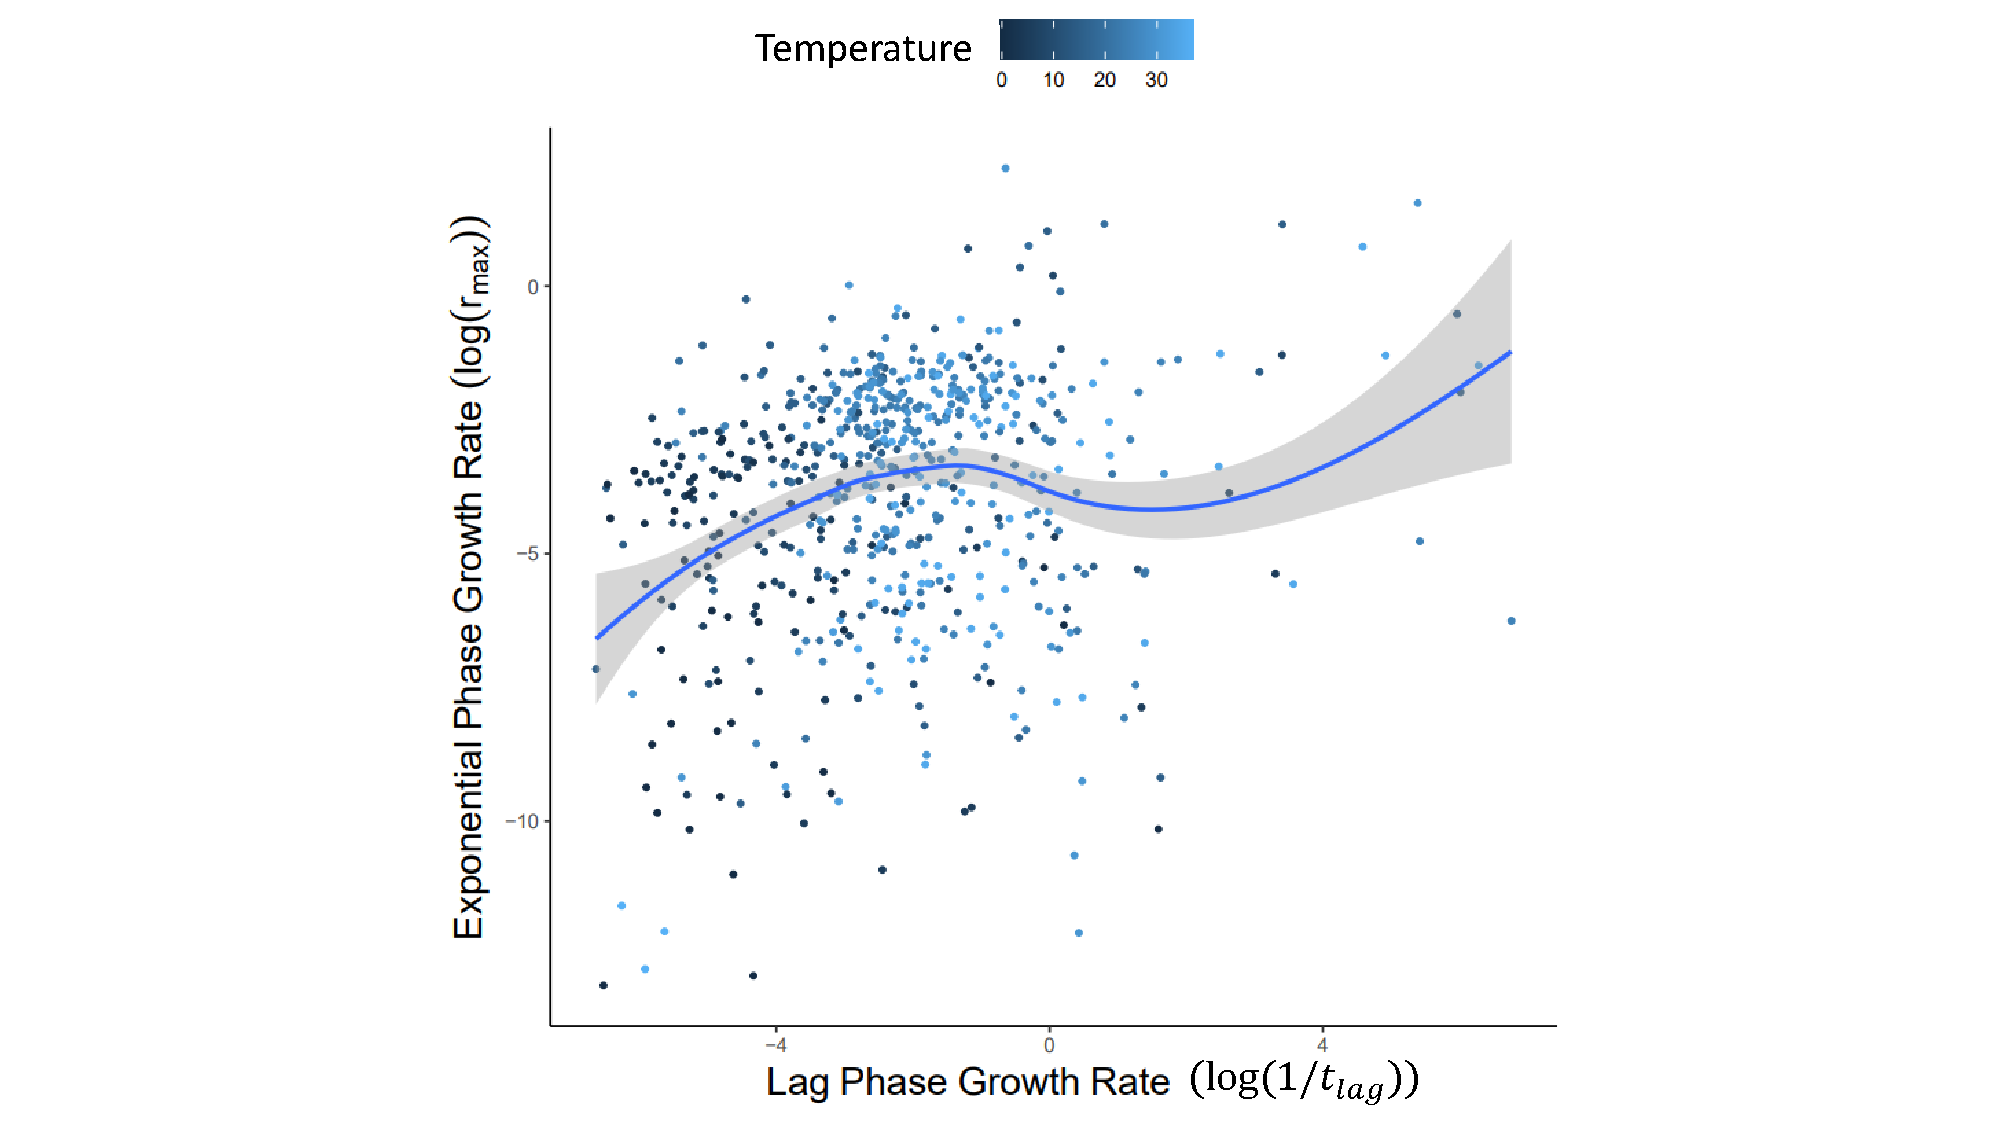
\includegraphics[width=1.1\linewidth]{Plot/log_rt_col_temp.pdf}
%\caption{Scater plot showing the relationship between \(P_{PK}\)(\(r_{max}\)) and %\(P_{lag}\)(\(1/t_{lag}\))}
%\label{fig:log_rt_temp}
%\end{figure}
%figure \ref{fig:log_rt_temp}, the result shows, the metabolic rates between lag and exponential phase do not have trade off, rather, they are positively correlated. \\